\subsubsection{Misleading SO \BRAVO sequences.} As we consider the idea of misleading samples, it is noteworthy that SO \BRAVO suffers from a different and unique type of misleading result. 

After drawing a cumulative $n>1$ ballots in a round, some number $k$ of them are votes for the announced winner. There are $\binom{n}{k}$ possible sequences of ballots which can lead to such a sample. Given a value of $k$, however, the particular sequence of the sample that led to that value of $k$ contains no additional information about whether the sample is more likely under the alternative or null hypotheses. That is to say, $\Pr[K=k|H_a]$ and $\Pr[K=k|H_0]$ have the same value regardless of the sequence.
Despite this, the SO \BRAVO RLA stopping condition is not just a function of $n$ and $k$ but also a function of the sequence, the selection order. In particular, if the sequence of ballots is such that the standard \BRAVO stopping condition was met for some $n'<n$ and corresponding $k'<n$, the audit will stop, even if by the end of the sequence the values $k$ and $n$ no longer meet the \BRAVO condition. We refer to such sequences which stop under SO \BRAVO, but not under EoR \BRAVO, as \emph{misleading sequences}. To be clear, this is not a mathematical issue; stopping in such cases is still a correct application of Wald's SPRT result\cite{wald}. The misleading nature of such stoppages is the note we are making. This is another case where election officials might have difficulty explaining the misleading situation to the public.

Recall from section~\ref{sec:pilot} that the pilot \Providence RLA performed in Providence, Rhode Island had an SO \BRAVO \emph{misleading sequence}. In particular, the audit passed with an SO \BRAVO risk measure of $0.0541$ but the final cumulative tally of the sample gives a \BRAVO risk measure of $0.366$.

It is easy to use our simulations to see how often SO \BRAVO \emph{misleading sequences} occur by checking whether the final cumulative sample of each SO \BRAVO trial meets the EoR \BRAVO stopping condition and counting those which do not. Figure~\ref{so_misleading} shows the proportion of simulated SO \BRAVO audits that stopped with a \emph{misleading sequence}. Unlike the more general \emph{misleading sample} discussed so far, these \emph{misleading sequences} are unique to SO \BRAVO audits, and Figure~\ref{so_misleading} only shows the proportion of audits that stopped with a \emph{misleading sequence}; additional SO \BRAVO audits also contained \emph{misleading samples}.

\begin{figure}
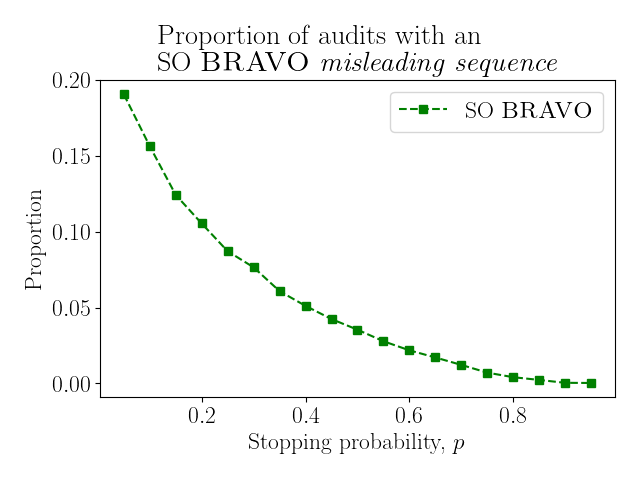
\includegraphics[width=.5\textwidth]{so_misleading.png}
\caption{The proportion of sequences that are misleading sequences in the SO \BRAVO audit as a function of $p$.}
\label{so_misleading}
\end{figure}




